% SOITCS Final Presentation
% Self-Organizing Systems 2025-2026
% Politehnica Bucharest

\documentclass[10pt, aspectratio=169]{beamer}

% Theme configuration
\usetheme{metropolis}
\metroset{
    titleformat=regular,
    sectionpage=progressbar,
    numbering=fraction
}

% Color customization - teal accent
\definecolor{SOITCSTeal}{RGB}{0, 128, 128}
\setbeamercolor{progress bar}{fg=SOITCSTeal, bg=SOITCSTeal!20}
\setbeamercolor{title separator}{fg=SOITCSTeal}
\setbeamercolor{frametitle}{bg=SOITCSTeal}
\setbeamercolor{alerted text}{fg=SOITCSTeal}

% Packages
\usepackage{tikz}
\usetikzlibrary{shapes, arrows.meta, positioning, fit, backgrounds}
\usepackage{booktabs}
\usepackage{multirow}
\usepackage{graphicx}
\usepackage{hyperref}
\usepackage[style=numeric, sorting=none, maxbibnames=2]{biblatex}

% Bibliography
\addbibresource{references.bib}

% Metadata
\title{SOITCS: Self-Organizing Intelligent Traffic Control Systems}
\subtitle{Self-Organizing Systems 2025--2026}
\author{Student Name}
\date{\today}
\institute{Politehnica University of Bucharest}

\begin{document}

% =============================================================================
% SLIDE 1: Title
% =============================================================================
\maketitle

% =============================================================================
% SLIDE 2: Introduction & Motivation
% =============================================================================
\begin{frame}{Introduction \& Motivation}
    \textbf{The Traffic Congestion Problem}
    \begin{itemize}
        \item Urban traffic congestion costs billions annually in lost productivity
        \item Traditional fixed-timing signals cannot adapt to dynamic conditions
        \item Incidents and rush-hour patterns cause cascading delays
    \end{itemize}

    \vspace{0.5cm}
    \textbf{Why Self-Organization?}
    \begin{itemize}
        \item Decentralized control enables local adaptation
        \item Emergent coordination without central authority
        \item Resilience to failures and changing conditions
    \end{itemize}
\end{frame}

% =============================================================================
% SLIDE 3: Project Goals
% =============================================================================
\begin{frame}{Project Goals}
    \begin{columns}[T]
        \begin{column}{0.5\textwidth}
            \textbf{Primary Objectives}
            \begin{enumerate}
                \item Integrate \alert{6 self-organizing algorithms} into a unified simulation
                \item Create an \alert{educational visualization} tool
                \item Demonstrate \alert{emergent behavior} in traffic systems
            \end{enumerate}
        \end{column}
        \begin{column}{0.5\textwidth}
            \textbf{Key Features}
            \begin{itemize}
                \item Real-time traffic flow simulation
                \item Interactive algorithm comparison
                \item Incident injection and response
                \item Performance metrics dashboard
            \end{itemize}
        \end{column}
    \end{columns}
\end{frame}

% =============================================================================
% SLIDE 4: State of the Art
% =============================================================================
\begin{frame}{State of the Art}
    \textbf{Foundational Approaches}

    \begin{description}
        \item[Cellular Automata] Nagel-Schreckenberg model (1992) captures realistic traffic flow with simple rules \cite{nagel1992cellular}

        \item[Self-Organizing Signals] SOTL by Cools et al. demonstrates adaptive control via local queue sensing \cite{cools2013sotl}

        \item[Swarm Intelligence] ACO and PSO applied to routing and signal optimization \cite{dorigo1997aco, kennedy1995pso}

        \item[Deep RL] Recent MARL approaches show promise for large-scale coordination \cite{chu2019marl}
    \end{description}

    \vspace{0.3cm}
    \alert{Gap:} Few systems integrate multiple paradigms for comparative study.
\end{frame}

% =============================================================================
% SLIDE 5: System Architecture
% =============================================================================
\begin{frame}{System Architecture}
    \begin{center}
    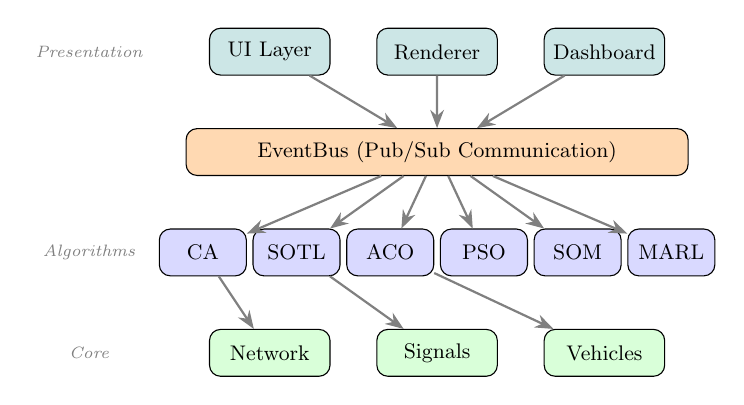
\begin{tikzpicture}[
        scale=0.85, transform shape,
        box/.style={rectangle, draw, rounded corners, minimum width=1.8cm, minimum height=0.7cm, align=center, font=\small},
        algobox/.style={rectangle, draw, rounded corners, minimum width=1.3cm, minimum height=0.7cm, align=center, font=\small},
        arrow/.style={-{Stealth}, thick}
    ]
        % Presentation Layer - centered at x=4
        \node[box, fill=SOITCSTeal!20] (ui) at (1.5, 3) {UI Layer};
        \node[box, fill=SOITCSTeal!20] (render) at (4, 3) {Renderer};
        \node[box, fill=SOITCSTeal!20] (dash) at (6.5, 3) {Dashboard};

        % EventBus - centered at x=4
        \node[box, fill=orange!30, minimum width=7.5cm] (bus) at (4, 1.5) {EventBus (Pub/Sub Communication)};

        % Algorithm Layer - 6 boxes evenly spaced from x=0.5 to x=7.5
        \node[algobox, fill=blue!15] (ca) at (0.5, 0) {CA};
        \node[algobox, fill=blue!15] (sotl) at (1.9, 0) {SOTL};
        \node[algobox, fill=blue!15] (aco) at (3.3, 0) {ACO};
        \node[algobox, fill=blue!15] (pso) at (4.7, 0) {PSO};
        \node[algobox, fill=blue!15] (som) at (6.1, 0) {SOM};
        \node[algobox, fill=blue!15] (marl) at (7.5, 0) {MARL};

        % Core Layer - 3 boxes centered at x=4 (Signals in middle to avoid crossing arrows)
        \node[box, fill=green!15] (net) at (1.5, -1.5) {Network};
        \node[box, fill=green!15] (sig) at (4, -1.5) {Signals};
        \node[box, fill=green!15] (veh) at (6.5, -1.5) {Vehicles};

        % Layer labels
        \node[font=\scriptsize\itshape, gray] at (-1.2, 3) {Presentation};
        \node[font=\scriptsize\itshape, gray] at (-1.2, 0) {Algorithms};
        \node[font=\scriptsize\itshape, gray] at (-1.2, -1.5) {Core};

        % Connections from presentation to bus
        \draw[arrow, gray] (ui) -- (bus);
        \draw[arrow, gray] (render) -- (bus);
        \draw[arrow, gray] (dash) -- (bus);

        % Connections from bus to algorithms
        \foreach \alg in {ca, sotl, aco, pso, som, marl} {
            \draw[arrow, gray] (bus) -- (\alg);
        }

        % Connections from algorithms to core
        \draw[arrow, gray] (ca) -- (net);
        \draw[arrow, gray] (sotl) -- (sig);
        \draw[arrow, gray] (aco) -- (veh);
    \end{tikzpicture}
    \end{center}

    \vspace{0.2cm}
    \begin{center}
    \small\textit{Event-driven architecture enables loose coupling and real-time coordination}
    \end{center}
\end{frame}

% =============================================================================
% SLIDE 6: Methodology - Algorithms Part 1
% =============================================================================
\begin{frame}{Methodology: The Six Algorithms (1/2)}
    \begin{columns}[T]
        \begin{column}{0.33\textwidth}
            \textbf{\alert{Cellular Automata}}
            \vspace{0.2cm}

            NaSch Model Rules:
            \begin{enumerate}
                \item Accelerate
                \item Brake for obstacles
                \item Random slowdown
                \item Move forward
            \end{enumerate}

            \textit{Realistic traffic flow from simple local rules}
        \end{column}

        \begin{column}{0.33\textwidth}
            \textbf{\alert{SOTL}}
            \vspace{0.2cm}

            Self-Organizing Signals:
            \begin{itemize}
                \item Monitor queue lengths
                \item Threshold-based switching
                \item Local adaptation only
                \item No global coordination
            \end{itemize}

            \textit{Emergent wave patterns}
        \end{column}

        \begin{column}{0.33\textwidth}
            \textbf{\alert{ACO}}
            \vspace{0.2cm}

            Ant Colony Routing:
            \begin{itemize}
                \item Pheromone trails
                \item Probabilistic path choice
                \item Evaporation mechanism
                \item Congestion avoidance
            \end{itemize}

            \textit{Distributed route optimization}
        \end{column}
    \end{columns}
\end{frame}

% =============================================================================
% SLIDE 7: Methodology - Algorithms Part 2
% =============================================================================
\begin{frame}{Methodology: The Six Algorithms (2/2)}
    \begin{columns}[T]
        \begin{column}{0.33\textwidth}
            \textbf{\alert{PSO}}
            \vspace{0.2cm}

            Signal Timing Optimization:
            \begin{itemize}
                \item Particles = timing configs
                \item Velocity updates
                \item Global/local best
                \item SOTL integration
            \end{itemize}

            \textit{Continuous parameter tuning}
        \end{column}

        \begin{column}{0.33\textwidth}
            \textbf{\alert{SOM}}
            \vspace{0.2cm}

            Pattern Recognition:
            \begin{itemize}
                \item Kohonen network
                \item Traffic state clustering
                \item Anomaly detection
                \item Visual state mapping
            \end{itemize}

            \textit{Unsupervised learning}
        \end{column}

        \begin{column}{0.33\textwidth}
            \textbf{\alert{MARL}}
            \vspace{0.2cm}

            Q-Learning Agents:
            \begin{itemize}
                \item One agent/intersection
                \item State: queue + phase
                \item Reward: throughput
                \item Neighbor awareness
            \end{itemize}

            \textit{Adaptive control policies}
        \end{column}
    \end{columns}
\end{frame}

% =============================================================================
% SLIDE 8: Algorithm Integration
% =============================================================================
\begin{frame}{Algorithm Integration}
    \textbf{EventBus Communication}

    \begin{center}
    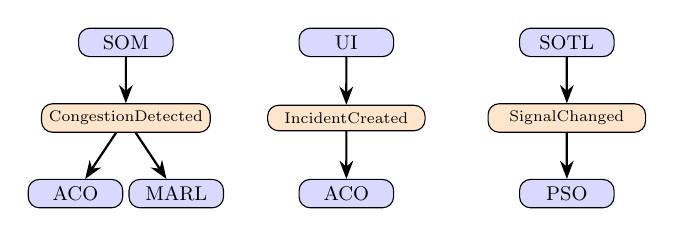
\begin{tikzpicture}[
        scale=0.8, transform shape,
        event/.style={rectangle, draw, rounded corners, fill=orange!20, font=\scriptsize, minimum width=2.5cm},
        algo/.style={rectangle, draw, rounded corners, fill=blue!15, font=\small, minimum width=1.5cm}
    ]
        % Events
        \node[event] (e1) at (0, 0) {CongestionDetected};
        \node[event] (e2) at (3.5, 0) {IncidentCreated};
        \node[event] (e3) at (7, 0) {SignalChanged};

        % Publishers
        \node[algo] (som) at (0, 1.2) {SOM};
        \node[algo] (ui) at (3.5, 1.2) {UI};
        \node[algo] (sotl) at (7, 1.2) {SOTL};

        % Subscribers
        \node[algo] (aco1) at (-0.8, -1.2) {ACO};
        \node[algo] (marl1) at (0.8, -1.2) {MARL};
        \node[algo] (aco2) at (3.5, -1.2) {ACO};
        \node[algo] (pso) at (7, -1.2) {PSO};

        % Arrows
        \draw[-{Stealth}, thick] (som) -- (e1);
        \draw[-{Stealth}, thick] (ui) -- (e2);
        \draw[-{Stealth}, thick] (sotl) -- (e3);

        \draw[-{Stealth}, thick] (e1) -- (aco1);
        \draw[-{Stealth}, thick] (e1) -- (marl1);
        \draw[-{Stealth}, thick] (e2) -- (aco2);
        \draw[-{Stealth}, thick] (e3) -- (pso);
    \end{tikzpicture}
    \end{center}

    \vspace{0.3cm}
    \textbf{Key Integrations:}
    \begin{itemize}
        \item \alert{SOTL + PSO}: PSO optimizes SOTL threshold parameters ($\theta$, $t_{\min}$, $t_{\max}$)
        \item \alert{SOM $\rightarrow$ ACO}: Pattern events trigger pheromone reduction (0.7$\times$ incident, 0.85$\times$ rush hour)
        \item \alert{SOM $\rightarrow$ SOTL}: Pattern events adjust timing multipliers (e.g., rush hour: $t_{\max} \times 1.3$)
        \item \alert{MARL + SOTL}: MARL learns when to override SOTL decisions
    \end{itemize}
\end{frame}

% =============================================================================
% SLIDE 9: Results - Visualization
% =============================================================================
\begin{frame}{Results: Visualization Features}
    \begin{columns}[T]
        \begin{column}{0.5\textwidth}
            \textbf{Multi-Layer Rendering}
            \begin{itemize}
                \item Road network with intersections
                \item Vehicle sprites with direction
                \item Traffic signal states
                \item ACO pheromone trails (heatmap)
                \item SOM cluster visualization
            \end{itemize}

            \vspace{0.3cm}
            \textbf{Interactive Controls}
            \begin{itemize}
                \item Algorithm toggle switches
                \item Incident injection (click)
                \item Simulation speed control
                \item Scenario presets
            \end{itemize}
        \end{column}

        \begin{column}{0.5\textwidth}
            \textbf{Real-Time Dashboard}
            \begin{itemize}
                \item Vehicle count and throughput
                \item Average speed metrics
                \item Per-algorithm statistics
                \item Congestion indicators
                \item Historical sparklines
            \end{itemize}

            \vspace{0.5cm}
            % Placeholder for screenshot
            \begin{center}
            \fbox{\parbox{0.8\textwidth}{\centering\vspace{1cm}\textit{[Screenshot of running simulation]}\vspace{1cm}}}
            \end{center}
        \end{column}
    \end{columns}
\end{frame}

% =============================================================================
% SLIDE 10: Results - Observations
% =============================================================================
\begin{frame}{Results: Key Observations}
    \begin{columns}[T]
        \begin{column}{0.5\textwidth}
            \textbf{Emergent Behaviors}
            \begin{itemize}
                \item Traffic ``green waves'' form naturally with SOTL
                \item ACO pheromones create dynamic load balancing
                \item MARL agents develop coordination strategies
            \end{itemize}

            \vspace{0.3cm}
            \textbf{Algorithm Comparison}
            \begin{itemize}
                \item SOTL: Fast adaptation, $-29\%$ delay
                \item ACO: Pheromone-guided routing, $-30\%$ delay
                \item SOM: Pattern detection enables integration
                \item Combined: $-44.5\%$ delay (synergistic)
            \end{itemize}
        \end{column}

        \begin{column}{0.5\textwidth}
            \textbf{Performance Metrics}

            \vspace{0.3cm}
            \begin{tabular}{@{}ll@{}}
                \toprule
                \textbf{Metric} & \textbf{Value} \\
                \midrule
                Frame Rate & 30 FPS \\
                Vehicle Capacity & 100--500 \\
                Grid Size & Up to 10$\times$10 \\
                Update Rate & 60 Hz \\
                \bottomrule
            \end{tabular}

            \vspace{0.5cm}
            \alert{Note:} Educational focus prioritizes visualization clarity over maximum scale.
        \end{column}
    \end{columns}
\end{frame}

% =============================================================================
% SLIDE 11: Results - Ablation Study (Additive)
% =============================================================================
\begin{frame}{Results: Ablation Study (Additive Contributions)}
    \textbf{Algorithm Contribution Analysis} (340 runs, 20 seeds $\times$ 17 configurations)

    \vspace{0.2cm}
    \begin{columns}[T]
        \begin{column}{0.48\textwidth}
            \textbf{Additive Contributions vs Baseline}\\
            {\small (CA-only baseline: $\bar{d} = 36.0$ ticks)}

            \vspace{0.2cm}
            \begin{tabular}{@{}lrll@{}}
                \toprule
                \textbf{Algorithm} & \textbf{$\Delta$ Delay} & \textbf{$p$-value} \\
                \midrule
                SOTL & $-29.4\%$ & $< 0.001^{***}$ \\
                \alert{ACO} & \alert{$-29.9\%$} & $< 0.001^{***}$ \\
                PSO & $-1.5\%$ & $0.12$ \\
                SOM & $0.0\%$ & -- \\
                \midrule
                Full Stack & $-44.5\%$ & $< 0.001^{***}$ \\
                \bottomrule
            \end{tabular}

            \vspace{0.2cm}
            {\small $^{***}p < 0.001$, Welch's $t$-test vs baseline}
        \end{column}

        \begin{column}{0.52\textwidth}
            \textbf{Subtractive Importance}\\
            {\small (delay impact when removed from full stack)}

            \vspace{0.2cm}
            \begin{tabular}{@{}lrl@{}}
                \toprule
                \textbf{Removed} & \textbf{$\Delta$ Delay} & \textbf{Sig.} \\
                \midrule
                $-$SOTL & $+30.4\%$ & $^{***}$ \\
                $-$ACO & $+36.7\%$ & $^{***}$ \\
                $-$PSO & $-7.6\%$ & $^{***}$ \\
                \alert{$-$SOM} & \alert{$+11.3\%$} & $^{***}$ \\
                \bottomrule
            \end{tabular}

            \vspace{0.2cm}
            {\small \alert{Key insight:} SOM contributes via event-driven integration with SOTL/ACO, not direct control.}
        \end{column}
    \end{columns}
\end{frame}

% =============================================================================
% SLIDE 12: Hyperparameters & Experimental Setup
% =============================================================================
\begin{frame}{Hyperparameters \& Experimental Setup}
    \begin{columns}[T]
        \begin{column}{0.5\textwidth}
            \textbf{Algorithm Hyperparameters}

            \vspace{0.1cm}
            {\scriptsize
            \begin{tabular}{@{}llr@{}}
                \toprule
                \textbf{Algorithm} & \textbf{Parameter} & \textbf{Value} \\
                \midrule
                \multirow{3}{*}{CA} & $v_{\max}$ & 5 cells/tick \\
                & $p_{\text{slow}}$ & 0.3 \\
                & lane change $\theta$ & 2 \\
                \midrule
                \multirow{3}{*}{SOTL} & $\theta$ (queue) & 5 \\
                & $\mu$ (platoon) & 3 \\
                & $[t_{\min}, t_{\max}]$ & $[10, 60]$ \\
                \midrule
                \multirow{3}{*}{ACO} & $\alpha$ (pheromone) & \alert{2.0} \\
                & $\beta$ (heuristic) & \alert{1.5} \\
                & $\rho$ (evaporation) & \alert{0.02} \\
                \midrule
                \multirow{3}{*}{PSO} & swarm size & 30 \\
                & $c_1, c_2$ & 2.0 \\
                & $w$ (inertia) & 0.7 \\
                \midrule
                SOM & grid size & $10 \times 10$ \\
                \bottomrule
            \end{tabular}
            }
        \end{column}

        \begin{column}{0.5\textwidth}
            \textbf{Experimental Protocol}

            \vspace{0.1cm}
            {\small
            \begin{itemize}
                \item \textbf{Duration:} 5400 ticks (3 min sim time)
                \item \textbf{Runs:} 20 per configuration
                \item \textbf{Seeds:} 0--19 (sequential)
                \item \textbf{Network:} $4 \times 4$ grid (48 roads)
                \item \textbf{Road length:} 15 cells
            \end{itemize}
            }

            \vspace{0.2cm}
            \textbf{Metrics Collected}
            {\small
            \begin{itemize}
                \item Average delay (ticks)
                \item Throughput (vehicles/tick)
                \item Average speed (cells/tick)
                \item Queue length at intersections
            \end{itemize}
            }

            \vspace{0.2cm}
            \textbf{Scenarios Tested}
            {\small
            \begin{itemize}
                \item Normal traffic ($\rho = 0.08$)
                \item Rush hour ($\rho = 0.15$)
            \end{itemize}
            }
        \end{column}
    \end{columns}
\end{frame}

% =============================================================================
% SLIDE 13: Conclusions
% =============================================================================
\begin{frame}{Conclusions}
    \textbf{Key Findings}
    \begin{itemize}
        \item \alert{SOTL and ACO} each reduce delay by $\sim$30\% independently
        \item \alert{Full stack integration} achieves 44.5\% delay reduction
        \item \alert{SOM's indirect contribution} (+11.3\% when removed) validates event-driven architecture
        \item Algorithm synergies: combined effect exceeds sum of individual contributions
    \end{itemize}

    \vspace{0.3cm}
    \textbf{Technical Contributions}
    \begin{itemize}
        \item Event-driven pub/sub architecture enabling loose algorithm coupling
        \item Tuned ACO hyperparameters ($\alpha=2.0$, $\beta=1.5$, $\rho=0.02$) for traffic domain
        \item SOM$\rightarrow$ACO/SOTL integration via \texttt{PATTERN\_RECOGNIZED} events
    \end{itemize}

    \vspace{0.3cm}
    \textbf{Future Work}
    \begin{itemize}
        \item Hyperparameter optimization via grid search / Bayesian methods
        \item Extended scenarios: multi-incident, varying network topologies
        \item Deep RL integration (DQN/PPO) for MARL component
    \end{itemize}
\end{frame}

% =============================================================================
% SLIDE 14: Questions
% =============================================================================
\begin{frame}[standout]
    Questions?

    \vspace{1cm}
    \small
    Code: \url{https://github.com/username/soitcs}
\end{frame}

% =============================================================================
% References
% =============================================================================
\begin{frame}[allowframebreaks]{References}
    \printbibliography[heading=none]
\end{frame}

\end{document}
